\section{Anhang}

\subsection{GANTT-Diagramme}
\subsubsection {Hardware-GANTT}
\begin{figure}[htbp]
	\centering
	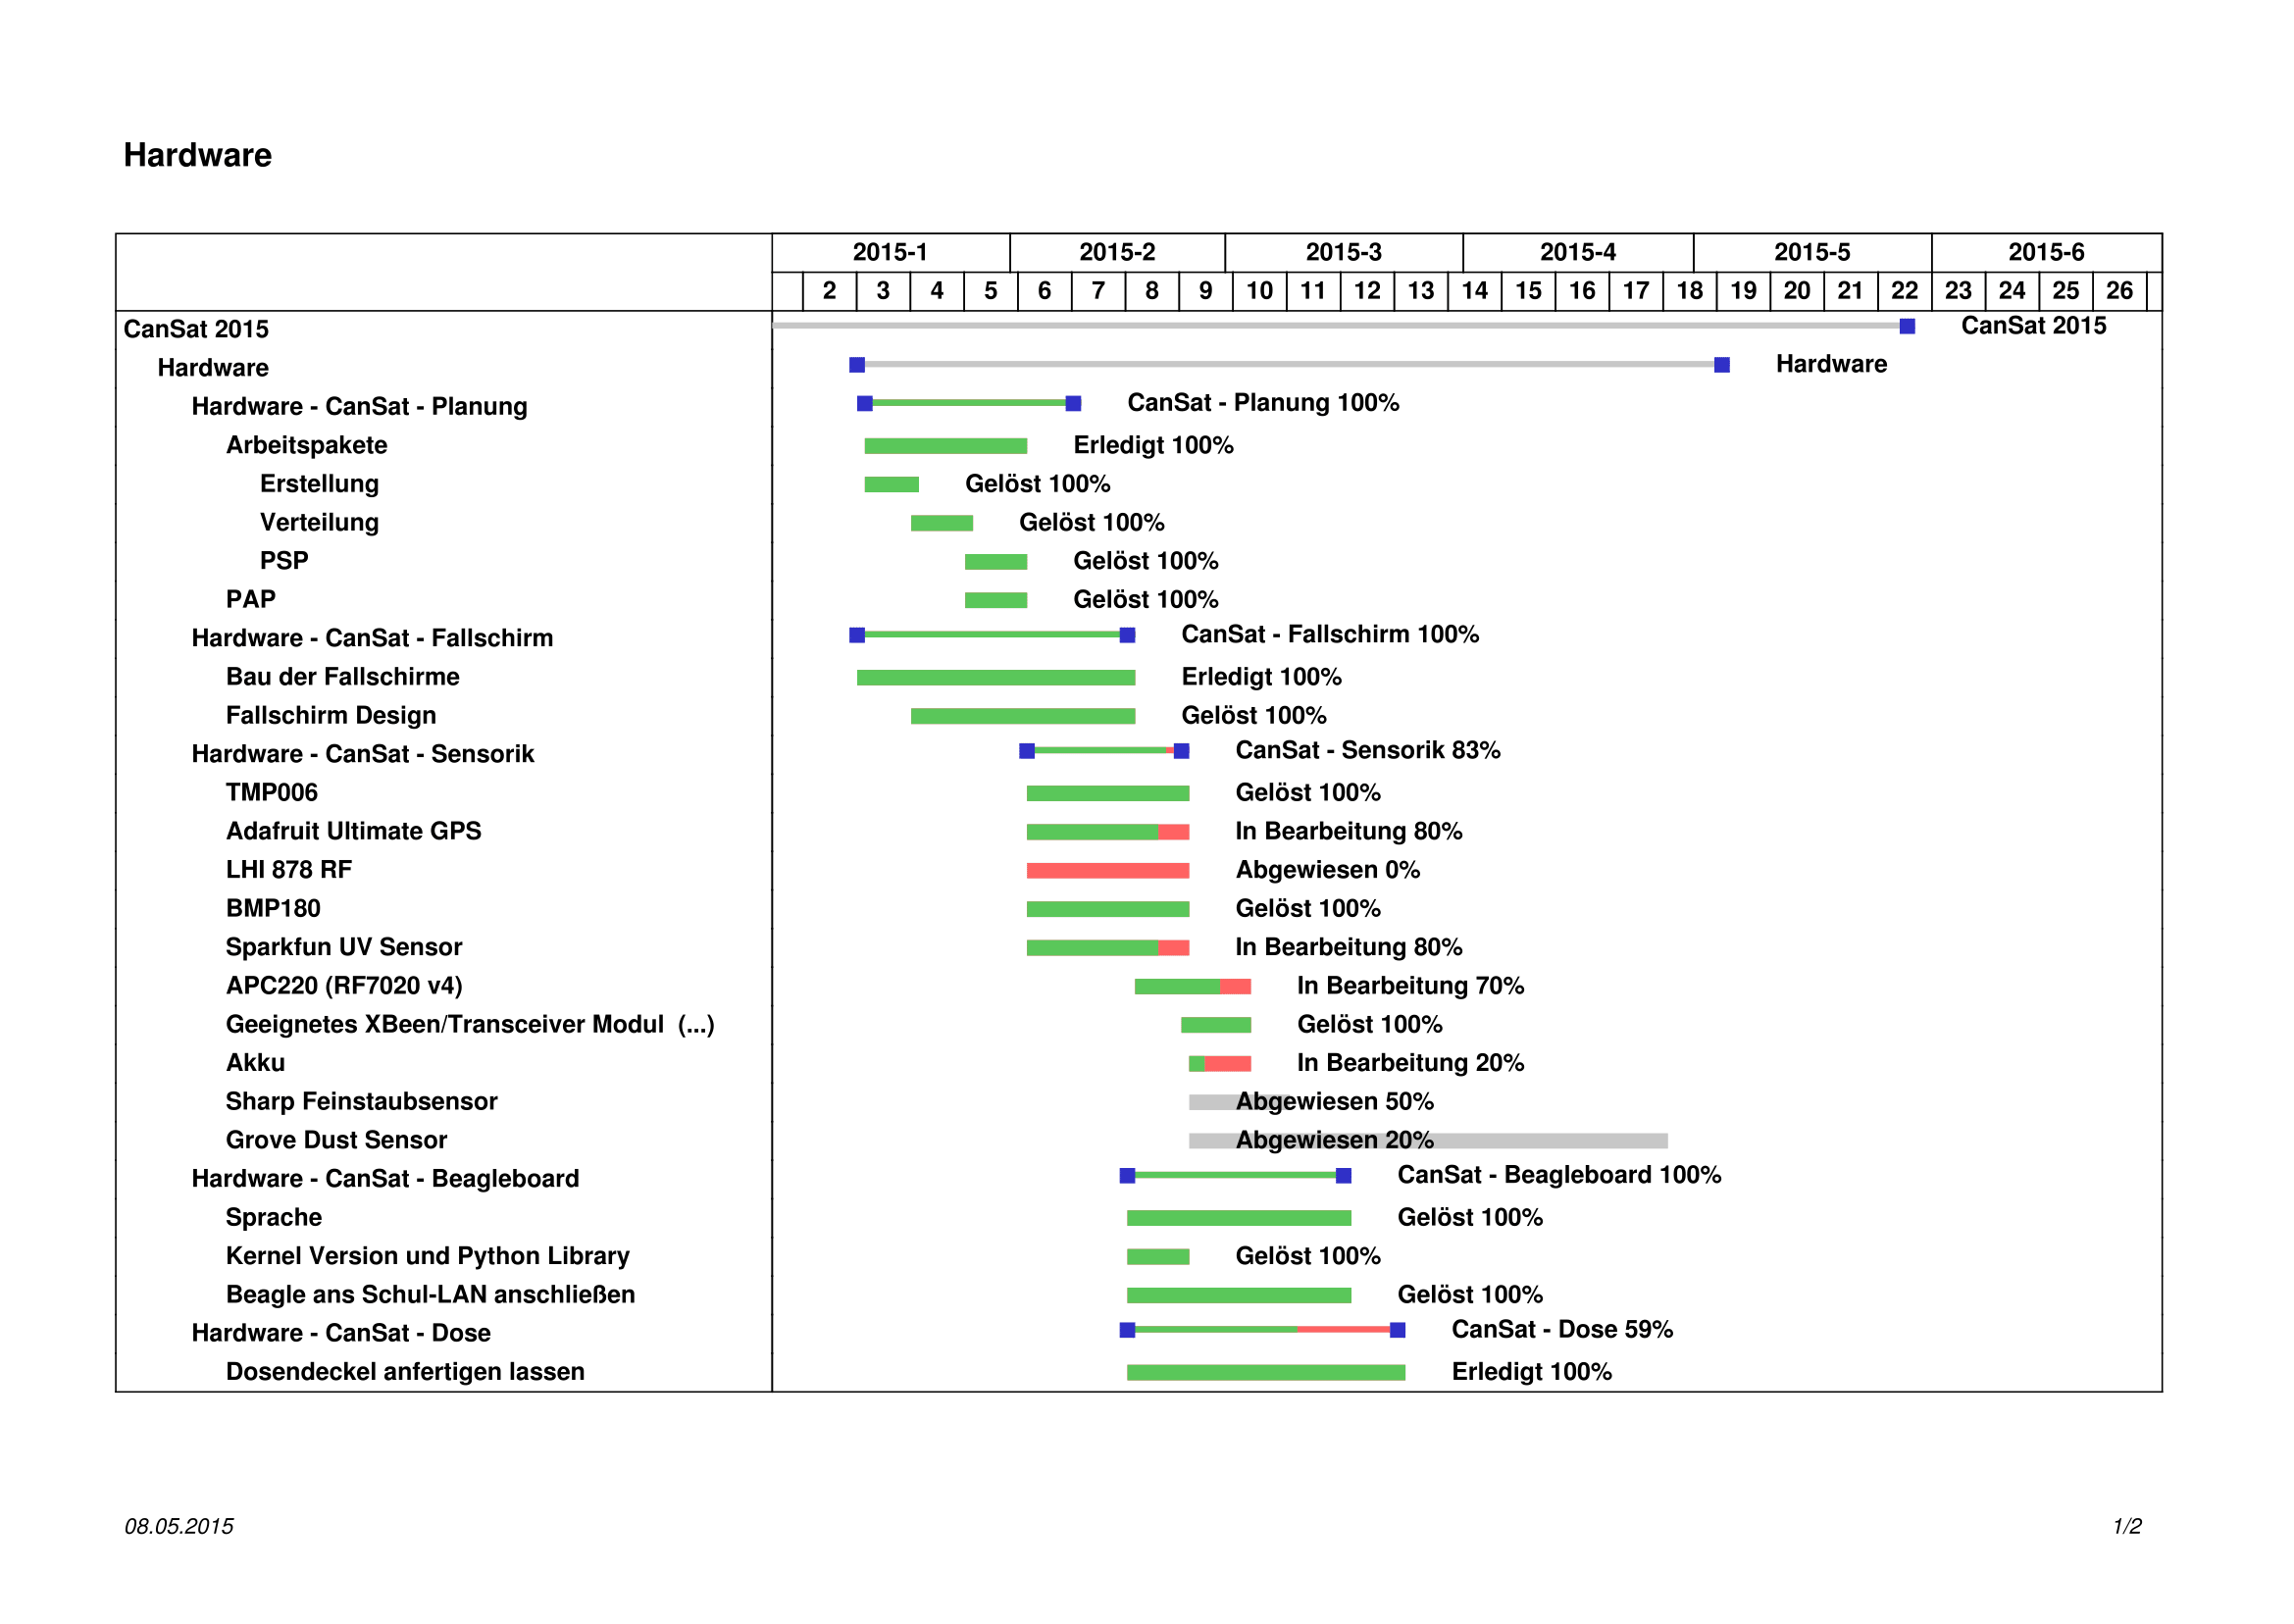
\includegraphics[trim = 10mm 50mm 20mm 65mm, clip,width=0.8\textwidth]{8_Anhang/hardware-gantt-1.png}
	\label{gantt_hardware_1}
\end{figure}
\vspace{-2cm}
\begin{figure}[htbp]
	\centering
	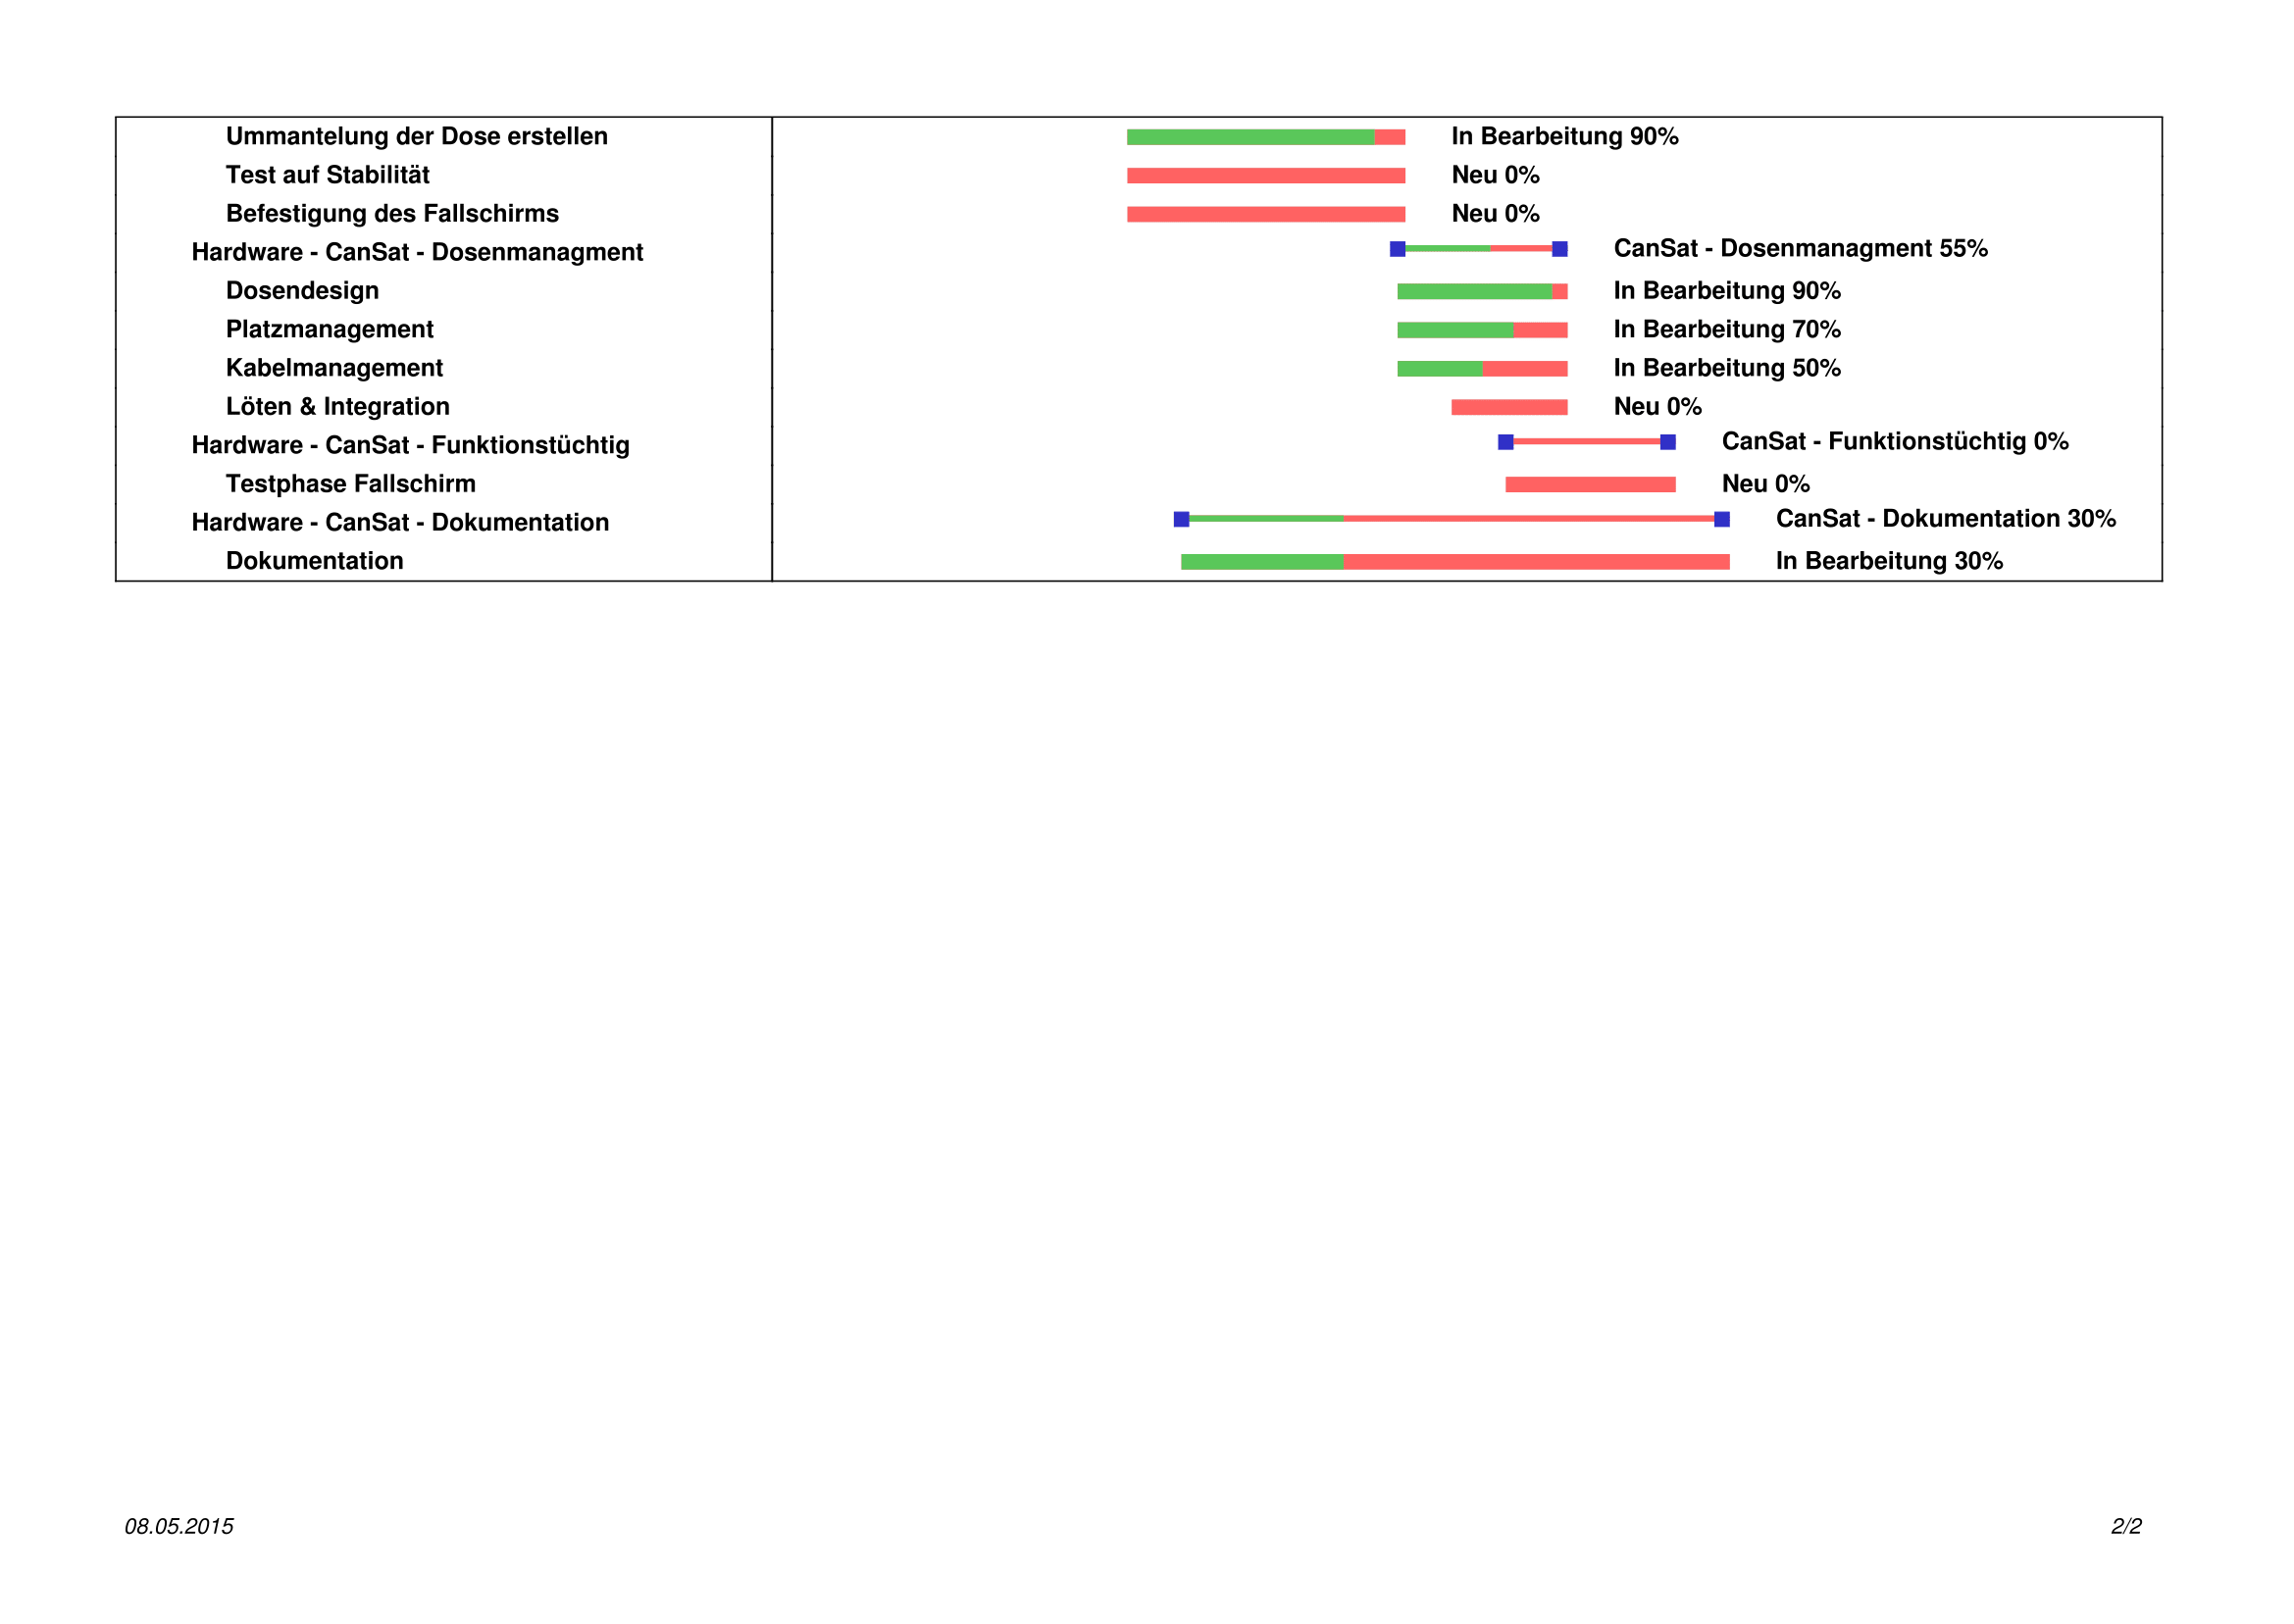
\includegraphics[trim = 11mm 350mm 20mm 40mm, clip,width=0.8\textwidth]{8_Anhang/hardware-gantt-2.png}
	\caption{Das GANTT-Diagramm der Hardware Gruppe}
	\label{gantt_hardware_2}
\end{figure}

\newpage
\subsection{Der CanSat}
\begin{figure}[h] 
      \centering 
      \includemovie[ 
        poster,controls,
       3Djscript=2_Beschreibung_des_CANSAT/Encompass.js
      ]{0.8\textwidth}{15cm}{2_Beschreibung_des_CANSAT/CanSat_2015.u3d} 
      \caption{Der Satellit (Diese Zeichnung ist möglicherweiße nicht sichtbar, da es eine 3D Zeichnung ist. Bitte verwenden sie den \href{https://get.adobe.com/reader/?loc=de}{Adobe Acrobat Reader})}\label{fig:hla} 
\end{figure} 

\newpage
\subsection{Bodenstationsarchitektur}
\begin{figure}[H]
	\centering
	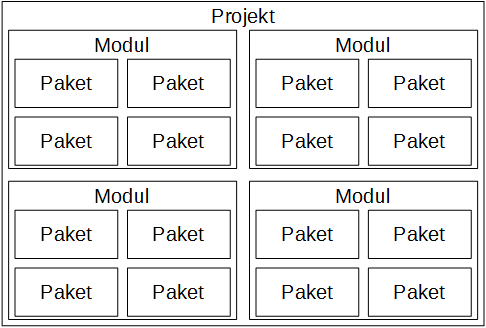
\includegraphics[width=0.8\textwidth]{3_Beschreibung_der_Bodenstation/NBP_Modularchitektur.png}
	\caption{Modularchitektur von Netbeans Platform}
	\label{nbp_modularchitektur}
\end{figure}

\begin{figure}[H]
	\centering
	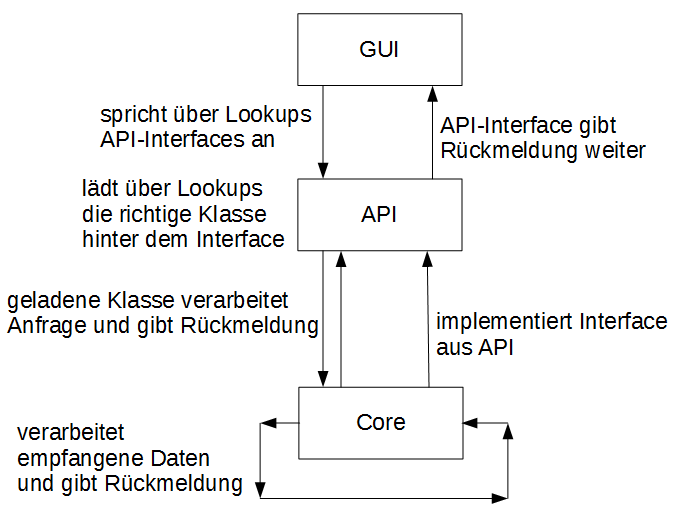
\includegraphics[width=0.8\textwidth]{3_Beschreibung_der_Bodenstation/Bodenstation_Modularchitektur.png}
	\caption{Modularchitektur der Bodenstation}
	\label{station_modularchitektur}
\end{figure}
\vspace{-5cm}
\newpage

\begin{figure}[H]
	\centering
	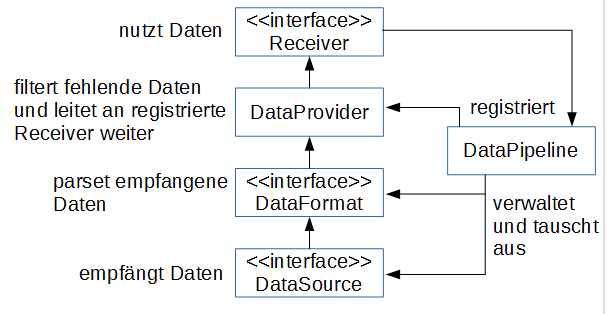
\includegraphics[width=0.8\textwidth]{3_Beschreibung_der_Bodenstation/Input-Pipeline_Architektur.png}
	\caption{Architektur der Input-Pipeline}
	\label{inputpipeline}
\end{figure}